\section{Stage 2: The good parts}

\begin{frame}[fragile]
  \begin{center}
    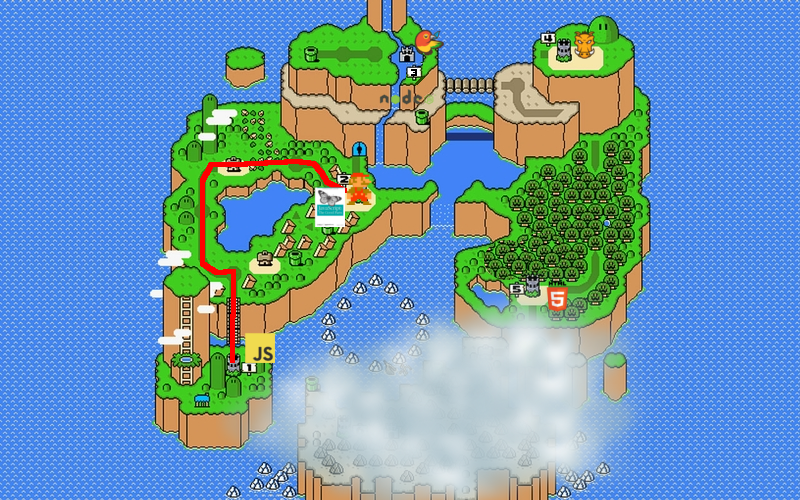
\includegraphics[width=300px]{images/map_stage_2.png}
  \end{center}
\end{frame}

\begin{frame}[fragile]
  \frametitle{Objects}
  \begin{itemize}
    \item Objects in Javascript are mutable keyed collections.
    \pause\item Arrays, functions and regular expressions are objects.
    \pause\item A property name can be any string.
    \pause\item Objects can inherit properties of another through its prototype.
  \end{itemize}

  \pause

  \begin{block}{\texttt{Prototype}}
    All objects created from object literals are linked to \texttt{Object.prototype}.
    \pause

    If we try to retrieve a property value from an object, and if the object lacks the property name, then Javascript attempts to retrieve the property value from the prototype object.
  \end{block}
\end{frame}

\begin{frame}[fragile]
  \frametitle{Objects}
  \begin{block}{\texttt{Object.create}}
    {\scriptsize
    \begin{verbatim}
    var soldier = {
        hp: 10,
        strength: 5,
        weapon: 'Pistol'
    };

    var knight = Object.create(soldier);
    knight.weapon = 'Sword';
    knight.shield = true;

    console.log(knight.hp); // Output: 10
    console.log(knight['weapon']); // Output: 'Sword'
    console.log(knight.shield); // Output: true
    \end{verbatim}
    }
  \end{block}

  Visit \url{http://www.objectplayground.com/} for a graphical explanation
\end{frame}

\begin{frame}[fragile]
  \frametitle{Objects}
  \begin{center}
    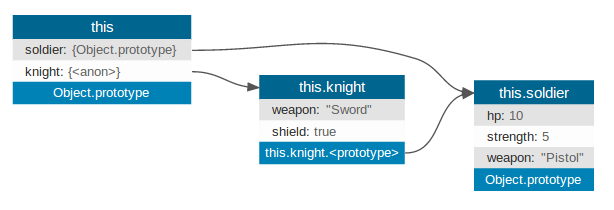
\includegraphics[width=300px]{images/object_create.png}
  \end{center}
\end{frame}

\begin{frame}[fragile]
  \frametitle{Objects}
  \begin{block}{\texttt{hasOwnProperty}}
    {\scriptsize
    \begin{verbatim}
    console.log(knight.hasOwnProperty('hp')); // Output: false
    console.log(knight.hasOwnProperty('shield')); // Output: true
    \end{verbatim}
    }
  \end{block}

  \pause

  \begin{block}{\texttt{for in}}
    {\scriptsize
    \begin{verbatim}
    for (attr in knight) {
        if(knight.hasOwnProperty(attr)) {
            console.log('Knight property ' + attr + ' with value ' + 
                knight[attr]);  
        }
    }
    // Knight property weapon with value 'Sword'
    // Knight property shield with value true
    \end{verbatim}
    }
  \end{block}
  
  \pause

  \begin{block}{\texttt{delete}}
    {\scriptsize
    \begin{verbatim}
    console.log(knight.weapon); // Output: 'Sword'
    delete knight.weapon;
    console.log(knight.weapon); // Output: 'Pistol'
    \end{verbatim}
    }
  \end{block}
\end{frame}

\begin{frame}[fragile]
  \frametitle{Functions}

  Functions are the \textbf{fundamental modular unit} of Javascript. They are used for code reuse, information hiding, and composition. \\

  The thing that is special about functions is that they can be invoked.
  \pause

  \begin{block}{Function.prototype}
  Functions are objects linked to Function.prototype.
  \end{block}
\end{frame}

\begin{frame}[fragile]
  \frametitle{Functions}
  \begin{center}
    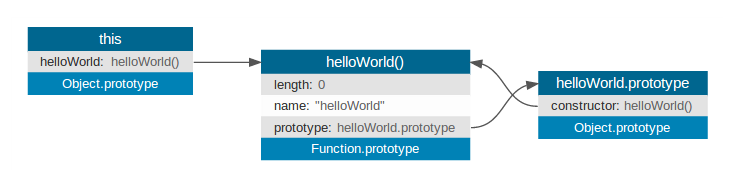
\includegraphics[width=300px]{images/function_prototype.png}
  \end{center}
\end{frame}

\begin{frame}[fragile]
  \frametitle{Functions}

  Invoking a function suspends the execution of the current function, passing control and parameters to the new function. In addition to the declared parameters, every function receives two additional parameters: \texttt{this} and \texttt{arguments}.

  \pause

  \begin{block}{\texttt{this}}
    Receive the value of the object invoking the function or the global object if it's called without an object.
  \end{block}

\end{frame}

\begin{frame}[fragile]
  \frametitle{Functions}
  \begin{block}{Invocation (1/4): Method invocation pattern}
    {\scriptsize
    \begin{verbatim}
    var enemy = {
        hp: 5,
        rage: 0,
        attack: function () {
            this.rage += 1;
        }
    };

    enemy.attack();
    console.log(enemy.rage); // Output: 1
    \end{verbatim}
    }
  \end{block}
\end{frame}

\begin{frame}[fragile]
  \frametitle{Functions}

  \begin{block}{Invocation (2/4): Function invocation pattern}
    {\tiny
    \begin{verbatim}
    physicsManager.collisionsDetected = 0;
    physicsManager.checkCollision = function (entity1, entity2) {
        var bbCollision = function (bb1, bb2) {
            // Collision code omitted
            var collision = true;
            if (collision) {
                // WARNING: 'this' is the global object and not 'physicsManager'
                this.collisionsDetected += 1;
            }
            return collision;
        };

        bbCollision(entity1.getBB(), entity2.getBB());
    };

    if (physicsManager.checkCollision(enemy, player)) {
        player.takeDamage(enemy.strength);
    }

    console.log(physicsManager.collisionsDetected); // Output: 0
    \end{verbatim}
    }
  \end{block}
\end{frame}

\begin{frame}[fragile]
  \frametitle{Functions}

  \begin{block}{Invocation (2/4): Function invocation pattern (workaround)}
    {\tiny
    \begin{verbatim}
    physicsManager.collisionsDetected = 0;
    physicsManager.checkCollision = function (entity1, entity2) {
        var that = this;

        var bbCollision = function (bb1, bb2) {
            // Collision code omitted
            var collision = true;
            if (collision) {
                that.collisionsDetected += 1;
            }
            return collision;
        };

        bbCollision(entity1.getBB(), entity2.getBB());
    };

    if (physicsManager.checkCollision(enemy, player)) {
        player.takeDamage(enemy.strength);
    }

    console.log(physicsManager.collisionsDetected); // Output: 1
    \end{verbatim}
    }
  \end{block}
\end{frame}

\begin{frame}[fragile]
  \frametitle{Functions}

  \begin{block}{Invocation (3/4): Constructor invocation pattern}
    {\scriptsize
    \begin{verbatim}
    var Player = function (name) {
        this.name = name;
        this.lives = 3;
    };

    Player.prototype.sayMyName = function () {
        console.log('My name is ' + this.name);
    };

    var david = new Player('David');
    david.sayMyName(); // Output: 'My name is David'
    \end{verbatim}
    }
  \end{block}
\end{frame}

\begin{frame}[fragile]
  \frametitle{Functions}
  \begin{center}
    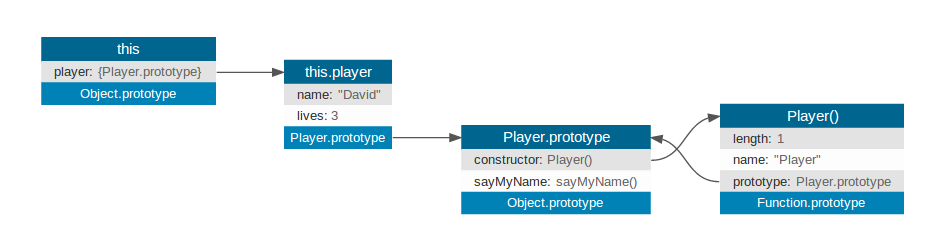
\includegraphics[width=300px]{images/basic_class.png}
  \end{center}
\end{frame}

\begin{frame}[fragile]
  \frametitle{Functions}

  \begin{block}{Invocation (3/4): Constructor invocation pattern (without new)}
    {\scriptsize
    \begin{verbatim}
    var Player = function (name) {
        this.name = name;
        this.lives = 3;
    };

    Player.prototype.sayMyName = function () {
        console.log('My name is ' + this.name);
    };

    var manfred = Player('Manfred'); // oops
    try {
        manfred.sayMyName(); // raise an error because manfred is undefined
    } catch (e) {
        console.log('[' + e.name + '] ' + e.message);
    }
    
    // Global variables feast
    console.log(name); // Output: 'Manfred'
    console.log(lives); // Output: 3
    \end{verbatim}
    }
  \end{block}
\end{frame}

\begin{frame}[fragile]
  \frametitle{Functions}

  \begin{block}{Invocation (4/4): Apply invocation pattern}
    {\scriptsize
    \begin{verbatim}
    var enemy = {
        rage: 0,
        attack: function () {
            this.rage += 1;
        }
    };

    var anotherEnemy = {
        rage: 10
    };

    enemy.attack.apply(anotherEnemy, []);

    console.log(anotherEnemy.rage); // Output: 11
    \end{verbatim}
    }
  \end{block}
\end{frame}

\begin{frame}[fragile]
  \frametitle{Functions}

  \begin{block}{\texttt{Arguments}}
  {\scriptsize
  \begin{verbatim}
  function doActions() {
      var i, l;

      // WARNING: arguments is an Array-like object
      for (i = 0, l = arguments.length; i < l; i += 1) {
          console.log('Doing action ' + arguments[i]);
      }
  }

  doActions('jump', 'attack');
  /*
      Output:
      'Doing action jump'
      'Doing action attack'
  */
  \end{verbatim}
  }
  \end{block}
\end{frame}

\begin{frame}[fragile]
  \frametitle{Functions}

  \begin{block}{Closure}
  Javascript does have function scope. That means that the parameters and variables defined in a function are not visible outside of the function, and that a variable defined anywhere within a function is visible everywhere within the function.
  {\scriptsize
  \begin{verbatim}
  var player = new Player();

  function isGameOver() {
      var enemy = new Enemy();

      function checkHit() {
          return enemy.hit(player);
      }

      return checkHit();
  }

  isGameOver();
  \end{verbatim}
  }
  \end{block}

\end{frame}

\begin{frame}[fragile]
  \frametitle{Functions}
  \begin{block}{Immediately-Invoked Function Expression (IIFE)}
  {\scriptsize
  \begin{verbatim}
  var something = (function () {
      // some code
  }());
  \end{verbatim}
  }
  \end{block}
\end{frame}

\begin{frame}[fragile]
  \frametitle{Functions}
  \begin{block}{Module pattern}
  {\tiny
  \begin{verbatim}
  var MYAPP = MYAPP || {};
  (function (exports) {
     var detectedCollisions = 0;

     function checkBBCollision(bb1, bb2) {
        // some code
     }

     function checkCollision(entity1, entity2) {
        checkBBCollision(entity1.getBB(), entity2.getBB());
     }

     exports.physicsModule = {
        checkCollision: checkCollision
     };
  }(MYAPP));
  \end{verbatim}
  }
  \end{block}
\end{frame}

\begin{frame}[fragile]
  \frametitle{Inheritance}

  Javascript provides a much richer set of code reuse patterns. It can ape the classical pattern, but it also supports other patterns that are more expressive.

  \pause

  \begin{block}{Javascript is a class-free language}
    In classical languages, objects are instances of classes, and a class can inherit from another class. Javascript is a prototypal language, which means that objects inherit directly from other objects.
  \end{block}
  
\end{frame}

\begin{frame}[fragile]
  \frametitle{Inheritance}

  \begin{block}{Pseudoclassical pattern}
  {\tiny
  \begin{verbatim}
  var Alien = function (name) {
      this.name = name;
  };

  Alien.prototype.talk = function () {
      console.log('%?saf? ' + this.name);
  };

  var SmartAlien = function (name) {
      this.name = name;
  };

  SmartAlien.prototype = new Alien();

  SmartAlien.prototype.speech = function () {
      this.talk();
      console.log('...I mean, my name is ' + this.name);
  };

  var enemy = new SmartAlien('Roger');
  enemy.speech(); 
  // Output: '%?saf? Roger
  //         ...I mean, my name is Roger'
  \end{verbatim}
  }
  \end{block}
\end{frame}

\begin{frame}[fragile]
  \frametitle{Functions}
  \begin{center}
    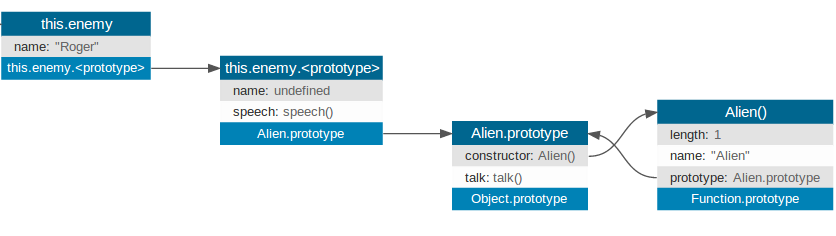
\includegraphics[width=300px]{images/classical_pattern.png}
  \end{center}
\end{frame}

\begin{frame}[fragile]
  \frametitle{Inheritance}

  \begin{block}{Prototypal pattern}
  {\tiny
  \begin{verbatim}
  var alien = {
      name: '%?&789',
      talk: function () {
          console.log('%?saf? ' + this.name);
      }
  };

  var smartAlien = Object.create(alien);
  smartAlien.speech = function () {
      this.talk();
      console.log('...I mean, my name is ' + this.name);
  };

  var enemy = Object.create(smartAlien);
  enemy.name = 'Roger';
  enemy.speech(); 
  // Output: '%?saf? Roger
  //         ...I mean, my name is Roger'
  \end{verbatim}
  }
  \end{block}
\end{frame}

\begin{frame}[fragile]
  \frametitle{Inheritance}

  \begin{block}{Functional pattern}
  {\tiny
  \begin{verbatim}
  var alien = function (spec) {                         var smartAlien = function (spec) {
      var that = {};                                        spec.weapon = 'Pistol'; // Private access
                                                            var that = alien(spec);
      var killHumans = function () { // Private access                                                             
        console.log('*Using ' + spec.weapon + '*');         that.speech = function () {
      };                                                        that.talk();
                                                                console.log('...I mean, my name is ' +
      that.talk = function () {                                   spec.name);
          console.log('%&78 ' + spec.name);                 };                                                       
          if (spec.weapon) {                                return that;
              killHumans();                             };
          }
      };

      return that;
  };

  var enemy = smartAlien({ name: 'Roger' });
  enemy.speech(); 
  // Output: '%?saf? Roger
  //         *Using Pistol*
  //         ...I mean, my name is Roger'
  \end{verbatim}
  }
  \end{block}
\end{frame}

\begin{frame}[fragile]
  \frametitle{Arrays}

  \begin{block}{Arrays doesn't exist}
  Javascript provides an object that has some array-like characteristics. It converts array subscripts into strings that are used to make properties.
  \end{block}

  \pause

  \begin{block}{Arrays literals}
  {\scriptsize
  \begin{verbatim}
  var enemies = [];

  console.log(enemies[9999]); // Output: undefined

  enemies[0] = 'Sigma';
  console.log(enemies[0]); // Output: 'Sigma'

  enemies[1] = 9000; // We can mix different types
  console.log(enemies[1]); // Output: 9000

  \end{verbatim}
  }
  \end{block}
\end{frame}

\begin{frame}[fragile]
  \frametitle{Arrays}

  \begin{block}{Remove elements}
  {\scriptsize
  \begin{verbatim}
  var enemies = ['Grassman', 'Bowser', 'Sephirot'],
      players = ['David', 'Manfred', 'Joanmi'];

  delete enemies[1]; // Bad idea
  console.log(enemies[1]); // Output: undefined
  console.log(enemies.length); // Output: 3

  players.splice(1, 1); // Yeah!
  console.log(players[1]); // Output: 'Joanmi'
  console.log(players.length); // Output: 2
  \end{verbatim}
  }
  \end{block}
\end{frame}
